\documentclass[handout]{beamer}

\usepackage{graphicx, subfigure}
\usepackage{amsmath}


% \usepackage{beamerthemesplit} // Activate for custom appearance

\title{\color{blue} Visual Perception and Mobility in Cities}
\subtitle{\color{magenta}Knowledge Lab Team Presentation}
\author{ Nandana Sengupta}
\date{\color{blue}\today}


\begin{document}






\frame{\titlepage}


\frame{
\frametitle{Overview}

\begin{itemize} \small
\item<2-> What are some visual characteristics of cities that may impact human mobility decisions? 
\begin{itemize}
\item<3-> Safety, Beauty, Wealth, Uniqueness
\end{itemize}

\item<4-> We can generate data on these rankings

\begin{itemize} \small
\item<5-> Using a voting platform:
 \item<6->
\includegraphics[width = 0.75\textwidth]{streetscore}
\item<7-> Using Deep Learning to extract image features.
\item<8-> Using active learning to present choices intelligently
\end{itemize}

\item<9-> But we also need data on \textit{how} people move in a city

\begin{itemize} \small
\item<10-> Cellphone data
\item<11-> GPS data
\end{itemize}


\end{itemize}

}




\frame{
\frametitle{Feature Extraction using Deep Learning Software}

\begin{center}

\textbf{Top 3 Predictors:} (office building, apartment building, hospital ) \\


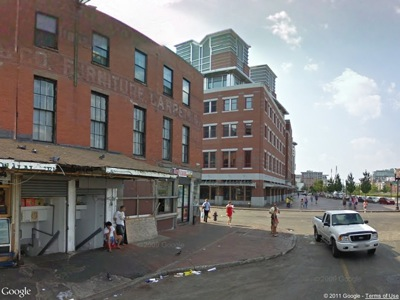
\includegraphics[width = 0.4\textwidth]{id_1_400_300.jpg}

\textbf{Top 3 Predictors:}(yard, residential neighborhood,  driveway) \\

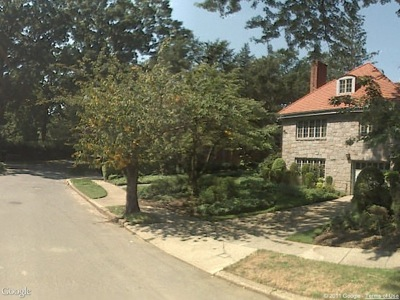
\includegraphics[width = 0.4\textwidth]{id_272_400_300.jpg}



\end{center}



}




\frame {


\frametitle{GPS Data from Spain}

\begin{itemize} \small
\item<1-> Human Mobility and Networks Lab at MIT -- PI Marta Gonsalez 

\item<2-> {\color{red}Paper:} ``Understanding individual routing
behaviour" (2016) -- Lima et el. 

\item<3-> {\color{red}Data:} anonymized GPS trajectories of personal cars over an 18-month period

\item<4-> {\color{red}Findings:}
\begin{itemize}  \small
\item<5-> most drivers tend to have a preferred route for frequent trips.
\item<6-> a significant fraction of drivers’ routes are not optimal from cost-minimization perspective
\end{itemize}

\item<7-> {\color{red}Open Question:} How are preferred routes characterized? Why do drivers choose economically suboptimal routes?
 \item<8-> \centering 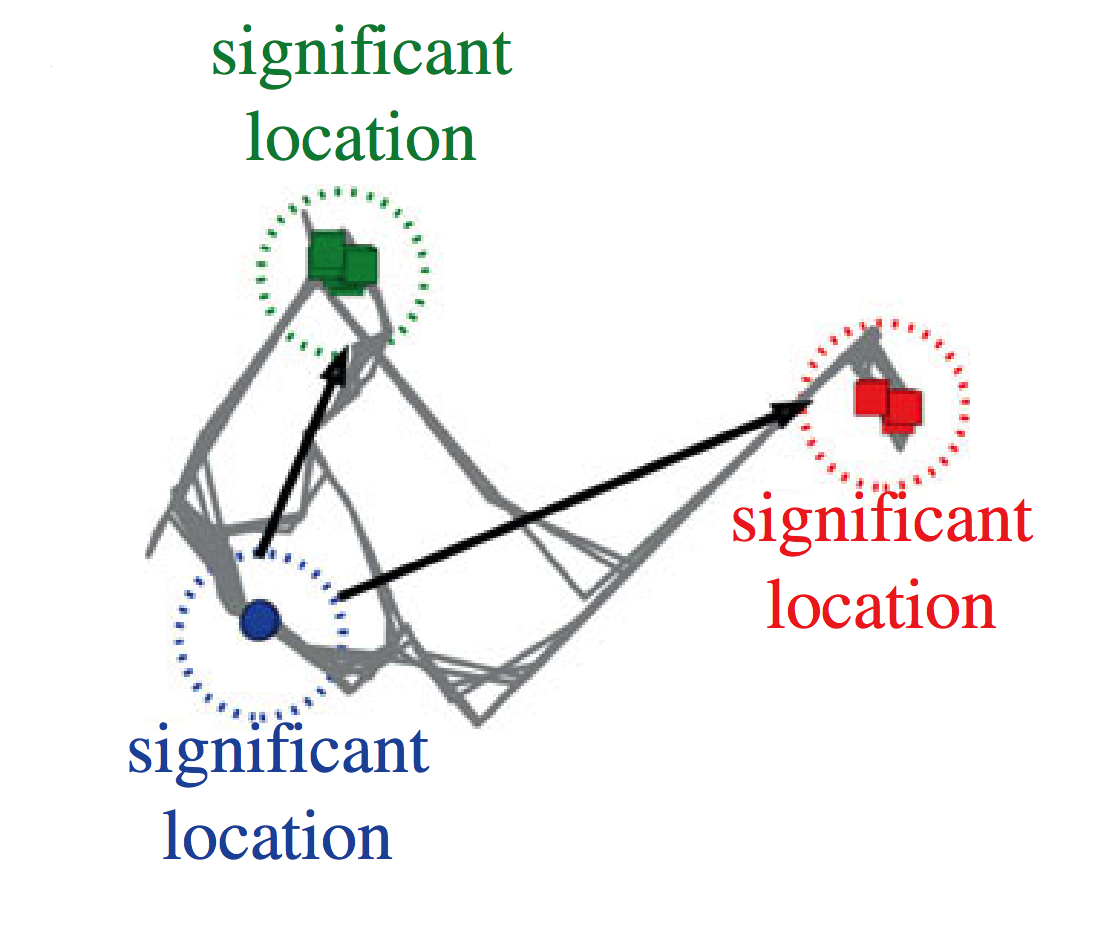
\includegraphics[width = 0.4\textwidth]{spain}


\end{itemize}



}




\frame {


\frametitle{Cellphone Data from Boston}

\begin{itemize} \small

\item<2-> {\color{red}Paper:} ``TimeGeo: a spatiotemporal framework for modeling urban mobility without surveys " (2016) -- Yang et al. 

\item<3-> {\color{red}Data:}  1.92 million anonymous mobile phone users, 6 weeks, Greater Boston area.
\item<4-> {\color{red}Findings:}
\begin{itemize}  \small
\item<5->  methodological: assign labels to \textit{`stay'} locations
\item<6-> provide origin destination matrices by converting sparse mobility traces into daily trajectories
\end{itemize}

\item<7-> {\color{red}Open Question:} What characterizes places where individuals cluster or linger?
 \item<8-> \centering 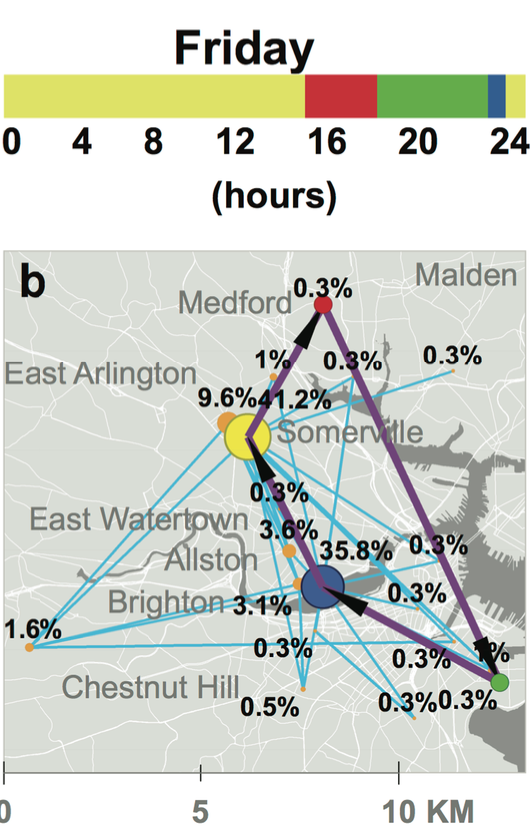
\includegraphics[width = 0.25\textwidth]{boston_mobile}


\end{itemize}

}



\frame{

\frametitle{Our Paper}

\begin{itemize} \small

\item<2->{\color{red} Aim: }Attempt to answer open questions from mobility data


\item<3->{\color{red} Methods:} Using Streetscore on images sampled from the locations in the GPS and cellphone datasets


\item<4-> {\color{red}Next Steps: }
\begin{itemize}
\item<5-> Setup an active learning interface on NEXTML 
\item<6-> Employ MTurkers to find streetscore ratings 
\item<7-> Get demographic and economic data corresponding to image locations
\item<8-> Estimate impact of visual characteristics on human mobility choices that aren't explained by demographic characteristics. 
\end{itemize}


\end{itemize}

}











\end{document}